\documentclass[12pt]{article}
\usepackage[margin=1in]{geometry}
\usepackage[all]{xy}
\usepackage{multicol}

\usepackage{amsmath,amsthm,amssymb,color,latexsym}
\usepackage{geometry}        
\geometry{letterpaper}    
\usepackage{graphicx}
\usepackage[shortlabels]{enumitem}
\usepackage[dvipsnames]{xcolor}
\usepackage[linktoc=all]{hyperref}

\newtheorem*{thm}{Theorem}
\newtheorem*{defn}{Definition}
\newtheorem*{cor}{Corollary}
\newtheorem*{prop}{Proposition}
\newtheorem*{lem}{Lemma}
\newtheorem*{rmk}{Remark}



\newcommand{\RR}{\mathbb{R}}
\newcommand{\NN}{\mathbb{N}}
\newcommand{\QQ}{\mathbb{Q}}
\newcommand{\FF}{\mathbb{F}}
\newcommand{\ZZ}{\mathbb{Z}}
\newcommand{\CC}{\mathbb{C}}
\newcommand{\ol}{\overline}
\newcommand{\AutG}{\text{Aut($G$)}}
\newcommand{\vp}{\vec{v}_p}
\newcommand{\f}{f:S\subset\CC\to\CC}
\newcommand{\q}[1]{\textbf{#1)}}
\newcommand{\ex}{Example }
\newcommand{\exs}{Examples }
\newcommand{\Hom}[2]{\text{Hom}(#1,#2)}
\definecolor{light-gray}{gray}{0.75}
\newcommand{\bra}[1]{\langle #1 \vert}
\newcommand{\ket}[1]{\vert #1 \rangle}
\newcommand{\braket}[2]{\langle #1\vert #2 \rangle}

\title{Introduction to Quantum Interactive Proof Systems and Applications}
\author{Liam Salt - APMA 990}
\begin{document}
	\maketitle
	
	\begin{abstract}
		In this paper, we introduce quantum interactive proof systems, demonstrate their advantages over classical systems, and showcase their utility by using them to prove certain properties of finite groups. We show that any language in PSPACE has a $2$-round quantum interactive proof system, which is strictly more powerful than the classical case. Finally, we consider quantum interactive proof systems in the context of group theory via the group non-membership problem. We show that succint proofs for non-membership are possible with a quantum proof system, which is impossible classically. Construction of efficient proofs for group non-membership also allows us to approach other group theoretical problems, such as: finding the maximal normal subgroup, and whether an integer N divides the order of a group.
	\end{abstract}
	\section{Introduction}
	
	\subsection{Some Computer Science Background}
	
	Before we can begin to define a quantum proof system, we first must introduce some classical computing formalism and terminology. In classical computing, an \textit{interactive proof system} is a Turing machine that encapsulates the mathematical idea of a proof. It models a proof as a sequence of communications between two actors: a potentially dishonest \textit{prover}, and a skeptical, honest \textit{verifier}. Through various \textit{rounds} of communication, the prover attempts to convince the verifier to accept their proof. The default convention is to assume the verifier is constrained to be a deterministic polynomial-time TM, whereas we make no constraints to the computational power of the prover. Additionally, an interactive proof system is assumed to satisfy both \textit{completeness} and \textit{soundess}, defined below:
	\begin{defn}
		An interactive proof system is said to be \underline{complete} or to satisfy completeness if for any true statement, the prover can always convince the verifier of its validity.
	\end{defn}
	\begin{defn} An interactive proof system is said to be \underline{sound} if for any false statement, the prover can only with negligible probability convince the verifier of its validity.
	\end{defn}

	\begin{rmk} Often, many of these conditions are loosened in various ways, e.g. the prover only needing to convince the verifier up to some probability.\end{rmk}
	
	Now we can more formally define a (deterministic) interactive proof system.\\
	
	We say that a formal language $L$ has a  deterministic $k$-round interactive proof system with error probability $\varepsilon$ with prover verifier pair $(P,V)$ if all of the following:
	\begin{enumerate}
		\item $(P,V)$ either accepts or rejects any input after $k$ rounds
		\item $\forall x\in L, (P,V)$ accepts $x$ with probability 1
		\item $\forall x\notin L, (P,V)$ accepts $x$ with probability $\varepsilon$ 
	\end{enumerate}
	
	Given this definition, a familiar, degenerate example is to show that any language in \textbf{NP} has a $1-$round interactive proof system with error probability $0$. We recall that one definition of \textbf{NP} is as the set of decision problems whose positive answers can be verified in polynomial time by a deterministic Turing machine. Accordingly, if a problem is in \textbf{NP}, then by definition on input our prover can produce a polynomial-sized certificate, which can be verified in polynomial-time exactly when the input is in the language. In fact, the class of languages which have a deterministic interactive proof system, termed \textbf{dIP}, is exactly equal to \textbf{NP}. We can think of this as meaning that we can capture the full power of deterministic interactive proof systems with the class \textbf{NP}.\\
	
	We can generalize the above definition by allowing the verifier to also have access to a random number generator, with which it may generate and make use of random bits in each round. The addition of the verifier's access to randomness brings us to the full definition of an interactive proof system. The complexity class of all languages that have interactive proof systems is termed \textbf{IP}, and it can be shown [potentially in this paper] that \textbf{IP}$=$\textbf{PSPACE}. In other words, problems which can be accepted by an interactive proof system are exactly those problems which require only polynomial-sized space (memory) to answer. 
	\subsection{Arthur-Merlin Protocol}
	Related to \textbf{IP}, is another class which will become important in the quantum case is \textbf{MA}, which stands for Merlin-Arthur (of King Arthur fame), and is comprised of languages which have a particular type of interactive proof system known as an Arthur-Merlin protocol. This class was originally described in \hyperref[bab]{[Bab85]} and \hyperref[gol89]{[Gol89]}.
	
	\begin{defn}
		A language $L$ is said to have an Arthur-Merlin protocol with prover-verifier pair (Merlin, Arthur) if:
		\begin{enumerate}
			\item Arthur has access to random bits $y\in B_m$, which are public (known to Merlin)
			\item If $x\in L$, then $\exists z\in B_n$ such that $P(\text{Arthur accepts }x|y,z)\geq \frac{2}{3}$.
			\item If $x\notin L$, then $\forall z\in B_n$ such that $P(\text{Arthur accepts }x|y,z)\leq\frac{1}{3}$. 
			\item $n,m$ are both polynomial-length
		\end{enumerate}
	
	
	\end{defn}
	Equivalently, we say $L\in \textbf{MA}$. For clarity, in the above definition $z$ is the polynomial-sized proof certificate provided by Merlin, and whether Arthur accepts Merlin's proof depends on both the string sent by Merlin and the random string produced by Arthur.\\
	
	The probability conditions given above are quite flexible. Given a language meeting the definition above, it can be shown that we can induce a new Arthur-Merlin pair for that language that achieves perfect completeness, and soundness with error probability at most $\frac{1}{2}$.\\
	
	It will be important to see how \textbf{MA} relates to other complexity classes:
	\begin{prop}\textbf{MA} contains both \textbf{NP}$=$\textbf{dIP} and \textbf{BPP}. \end{prop}
	\begin{proof}The second containment is easy to see given the definition of \textbf{BPP}, as Arthur has access to random bits and a polynomial-time Turing machine (with acceptance prob $\frac{2}{3}$ as required in \textbf{BPP}); therefore, Arthur need not send anything to Merlin, as he is capable of solving any problem in \textbf{BPP} himself.\\Similarly for \textbf{NP}, Merlin can solve the problem then send Arthur the proof certificate which he can verify deterministically, i.e. without needing his random bits. \end{proof}
	
    \section{Quantum Interactive Proof Systems}
    Now that we have seen the definition of interactive proof systems in the classical case, we can discuss what happens if we allow the Turing machines access to quantum computations. It has been observed that allowing access to quantum computation lends itself to significant speed-up in many classical problems, including: from integer factorization, computing discrete logarithms, efficient unstructured search, etc., so it makes sense to ask whether any of the above definitions in section 1 are significantly affected by access to quantum circuits.
   
    \begin{rmk}The Turing machine model is sufficient, but for the remainder of this paper we will use the equivalent circuit model of quantum computation. \end{rmk}
    
    Specifically, a quantum interactive proof system is one where the verifier has access to quantum circuits which can solve problems in \textbf{BQP}, while the prover is still unrestricted (within the boundaries of quantum mechanics). The convention is for the messages exchanged between prover and verifier to be encoded as quantum states in the usual $n-$qubit $z-$basis. Some relevant terminology is that we call the class of all languages that have quantum interactive proof systems Quantum \textbf{IP} or \textbf{QIP}.
    \begin{defn}
    	A language $L$ is said to have a quantum interactive proof system with error probability $\varepsilon$, or to be in \textbf{QIP}, if:
    	\begin{enumerate}
    		\item The verifier accepts or rejects any input $x$ using a quantum circuit solving problems in \textbf{BQP}.
    		\item If $x\in L$, then given the polynomial-many actions of the prover, the verifier accepts $x$ with probability $1$.
    		\item If $x\notin L$, then regardless of the actions of the prover, the verifier accepts $x$ with probability $\varepsilon$.
    	\end{enumerate}
    \end{defn}

	We can see that this definition for \textbf{QIP} looks quite similar to the classical definition of \textbf{IP}, which we discuss more in the next section. In its current state \textbf{QIP} is actually only as powerful as \textbf{IP}, and in fact, \textbf{QIP}=\textbf{IP}=\textbf{PSPACE}. 
	\subsection{Relationship between QIP and PSPACE}
	Despite the simplicity of the claim at the end of the previous section, we can say a bit more about the relationship between \textbf{QIP} and \textbf{PSPACE}. Namely, we can put a very nice bound on the number of queries required in a quantum interactive proof system to determine any language in \textbf{PSPACE}. We introduce the first theorem, which is the principal subject of \hyperref[wat99]{[Wat99]}:
	\begin{thm}
		Every language in \textbf{PSPACE} has a $2-$round quantum interactive proof system with exponentially small error probability. 
	\end{thm}

	In other words, we can prove that \textbf{PSPACE} $\subseteq$ \textbf{QIP[2]}, the class of languages with $2-$round quantum interactive proof systems, a much tighter bound than what was claimed in the previous section. Importantly, this also shows that in the constant round case, \textbf{IP[k]} is strictly outperformed by \textbf{QIP[2]}, demonstrating the power of moving to quantum computations.\\
	
	To prove the above theorem, we need to show that any language in \textbf{PSPACE} has such a proof system, but it will be sufficient to prove the theorem for a language which is \textbf{PSPACE}-complete. In particular, we show the theorem for the language of true quantified boolean formulas, that is the language of true expressions $Q_1x_1\cdots Q_nx_nf(x_1,\dots,x_n)$, where $Q_i$ is a universal or existential quantifier $(\forall,\exists)$, $x_i$ are boolean valued variables, and $f$ is a boolean formula $B_n\to B$ consisting of operations $\wedge,\vee,\neg$,etc on the variables $x_1,\dots,x_n$. \\
	
	There is a classical protocol outlining an interactive proof system for the QBF problem \hyperref[she92]{[She92]}, but this is general takes $N={{n+1}\choose{2}}+n$ rounds of communication. A full description of this classical protocol is not shown in this paper, but it is outlined in \hyperref[wat99]{[Wat99]}:
	
	\noindent A general outline of the algorithm for a formula $Q$ is:
	 \begin{enumerate}
	 	\item The verifier sends the prover a random element $r_1$ of a finite field, and gets a corresponding function $f_1$ in response from the prover.
	 	\item They continue this exchange $N$ times, with each response polynomial $f_i$ being at most $\deg d$ and  depending only on the previously received random elements $r_1,\dots,r_{i}$. 
	 	\item After receving  the final $f_N$, the verifier inputs all of the data they have collected into a single predicate: $E(Q,r_1,\dots,r_N,f_1,\dots,f_N)$
	 	\item The verifier accepts if and only if $E(Q,r_1,\dots,r_N,f_1,\dots,f_N)$ evaluates to true.
	 \end{enumerate}
	 	
	After some analysis, this serves to prove that in the classical case, \textbf{IP}=\textbf{PSPACE}, and we therefore have already that \textbf{PSPACE}$\subseteq$\textbf{QIP}, as we can simulate the classical circuit in the quantum case. Thus, it remains to show that allowing our system access to quantum circuits helps to reduce the number of rounds.\\
	
	Now, we outline a $2-$round quantum protocol for the language of true quantified boolean formulas. \\
	
	We construct a quantum circuit which consists of three collections of registers: $\textbf{R}_{i,j},\textbf{S}_{i,j},$ and $\textbf{F}_{i,j}$, for $1\leq i\leq m$ and $1\leq j\leq N$, where $N={{n+1}\choose{2}}+n$ as above, and $m=q(n)$ for some polynomial $q$. The $mN$ registers found in the collections $\textbf{R}$ and $\textbf{S}$ each consist of $k$ qubits, where $\mathbb{F}_{2^k}$ is some chosen finite field (In the classical protocol, a finite field is chosen such that it is as large as computationally practical, as the error rate goes down exponentially in $k$). Each register in $\textbf{F}$ consists of $k(d+1)$ qubits, where $d$ is the total length of the inputted formula. Each $F_{i,j}$ represents a polynomial of degree at most $d$ with coefficients in $\mathbb{F}_{2^k}$, for example if $d=3$ and $k=2$, we represent the polynomial $3x^3+2x+1$ as:
	\[3x^3+x+1\to \ket{11}\ket{00}\ket{10}\ket{01}\]
	Additionally, the verifier needs to store classically the value of a vector $u\in\{1,\dots,N\}^m$. According to the vector $u$, we partition the collections $R$ and $F$ into two parts:
	\[R^{(u)}=\{R_{i,j}|j\in\{1,\dots,u_i-1\}\}, \overline{R^{(u)}}=R \setminus R^{(u)}\]
	\[F^{(u)}=\{F_{i,j}|j\in\{1,\dots,u_i\}\}, \overline{F^{(u)}}=F \setminus F^{(u)}\]
	
	To summarize, we have defined three 2D arrays of registers, and partitioned two of them according to a vector. An example of \textbf{R} and \textbf{F} with $N=8$, $m=5$, and $u=(7,6,3,2,5)$ is shown below:
	\begin{figure}[h!]
		\centering
		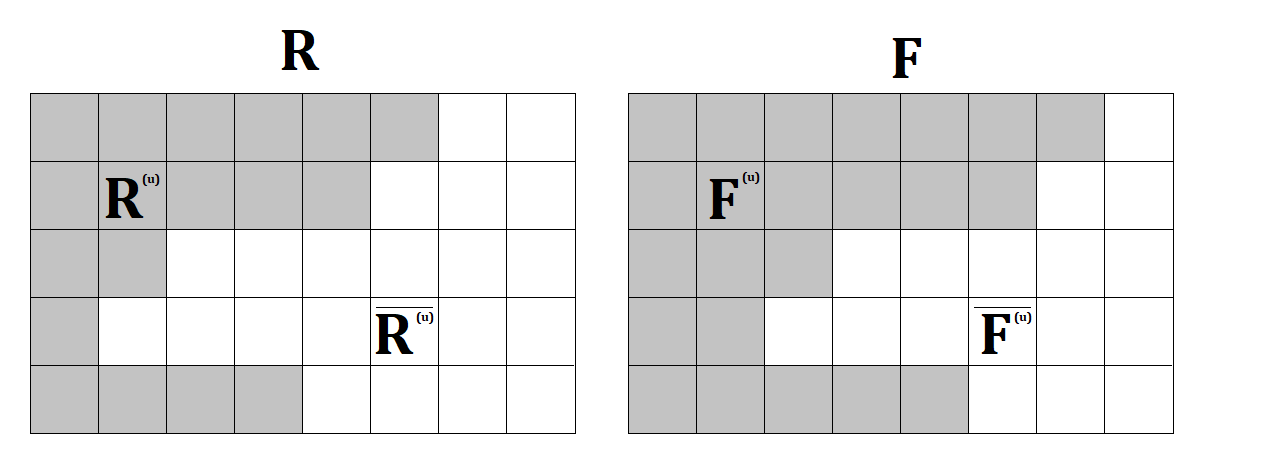
\includegraphics[width=\linewidth]{R grid.png}
	\end{figure}
	
	The protocol proceeds as follows: First, the prover sends \textbf{R}, and \textbf{F} which they calculate using their unlimited computing power. Then, using the classical verification protocol described in \hyperref[she92]{[She92]} for each pair of rows in the above table (\textbf{R}$_i$,\textbf{F}$_i$), the verifier rejects the proof if any pair for $i=1,\dots,m$ contain an invalid proof that the input formula evaluates to true. The verifier chooses vector $u$ uniformly randomly from $\{1,\dots,N\}^m$ and sends it to the prover along with $\overline{\textbf{F}^{(u)}}$. In the second round, the prover sends $S$ to the verifier, and they calculate \textbf{R}$_{i,j}$-\textbf{S}$_{i,j}$ for each pair $(i,j)$. Finally, the verifier applies $H^{\otimes k}$ to each register of $\overline{\textbf{R}^{(u)}}$ and accepts if and only if $\overline{\textbf{R}^{(u)}}$ contains only zeros.\\
	
	Some notes: the entries in $\textbf{R}$ and $\textbf{F}$ correspond to the random values $r_i$ and functions $f_i$ from the classical protocol. A full proof of correctness is found in \hyperref[wat99]{[Wat99]}, but we provide an outline here.
	
	\begin{proof}
		First suppose that a given formula $Q$ is true. We want to show that the verifier accepts it with certainty. The prover also creates a random $m\times N$ matrix $R$ of values in $\mathbb{F}_{2^k}$, where $m,N,$ and $k$ are defined as above. Using the values of $R$, the prover also generates a corresponding $m\times N$ matrix of correct polynomials $C(R)$. Each row $C(R)_i$ is formed by defining polynomials $f_{i,j}$ as in the classical protocol, where instead of getting the random values $r_j$ from the verifier, they are taken from the corresponding row $R_i$ of the generated matrix $R$. Thus, $C(R)_{i,j}=f_{i,j}(R_{i,1},\dots,R_{i,N})$, for $i=1,\dots,m,j=1,\dots,N$. The prover then prepares the following state:
		\[\frac{1}{\sqrt{2^{kmN}}}\sum_{i,j}\ket{R_{i,j}}\ket{C(R)_{i,j}}\]
		
		Forming the registers \textbf{R} and \textbf{F} as in the above protocol $\textbf{R}_{i,j}$ to $\textbf{S}_{i,j}$. The prover then sends this state to the verifier. As we are assuming $Q$ is true, the honest verifier will not reject at this point, and they will return $\overline{\textbf{F}^{(u)}}$ and $u$ to the verifer in response. Then, for each $(i,j)$ define a unitary:
		\[U_{i,j}:\ket{R}\ket{0}\mapsto\ket{R}\ket{C(R)_{i,j}}\]
		The prover then applies $U_{i,j}^{-1}$ to registers $\textbf{S}_{i,j}$ and $F_{i,j}$ for all $F_{i,j}$ in $\overline{\textbf{F}^{(u)}}$, which keeps $\textbf{S}$ the same, but returns all of $\overline{\textbf{F}^{(u)}}$ to $\ket{0}$. After the verifier subtracts each \textbf{R}$_{i,j}$ from each \textbf{S}$_{i,j}$, the registers in $\overline{\textbf{R}^{(u)}}$ will no longer be entangled with any other registers; therefore each register in $\overline{\textbf{R}^{(u)}}$ is sent to the zero state, and the verifier will accept $Q$ with certainty.\\
		In the case where $Q$ is not a true formula, the verifier will accept with some error probability. An upper bound for this probability is determined by $m$ and $k$. If we choose $m=(d+1)N$ and $k=2d+6+\lceil\log(dm\rceil)$, then $\varepsilon<2^{-d}$, i.e. the error probability is exponentially small in the length of $Q$.
	\end{proof}
	
	\noindent Therefore, we have proved that \textbf{PSPACE}$\subseteq$\textbf{QIP[2]}; moreover, there is an $\varepsilon<2^{-|x|}$ protocol for any language $L$ in \textbf{PSPACE}.  
	\subsection{QMA}
	Having now introduced quantum interactive proof systems and the classical class \textbf{MA}, we can discuss its natural extension \textbf{QMA}.
	\begin{defn}
		A language $L$ is in said to be in the class \textbf{QMA} if there exists a family of polynomial-time quantum circuits such that:
		\begin{enumerate}
			\item If $x\in L$, then there exists a state $\ket{\Psi}$ such that $P(\text{Circuit accepts } \ket{\Psi})>\frac{2}{3}$
			\item If $x\notin L$, then for any state $\ket{\Psi}$, $P(\text{Circuit accepts } \ket{\Psi})<\frac{1}{3}$
		\end{enumerate}
	\end{defn}
	 There are several important results to do with this class. For example, it has been shown by Kitaev that \textbf{QMA}$\subseteq$\textbf{P$^{\sharp P}$}\hyperref[kit99]{[Kit99]}. Another result of Marriott and Watrous is that \textbf{QMA}$\subseteq$\textbf{PP}\hyperref[mar05]{[Mar05]}, and further, if the reverse containment holds and \textbf{QMA}=\textbf{PP}, it can be shown that \textbf{PH}$\subseteq$\textbf{PP}\hyperref[vya03]{[Vya03]}.
    \section{Group Theoretic Applications}
    Having introduced it in the previous section, we proceed to discuss \textbf{QMA} in the context of group theory. The principal result of \hyperref[wat00]{[Wat00]} is a proof of the fact that the group non-membership problem is in \textbf{QMA}. This section will review the proof of this fact, along with some corollaries that allow us to recover various other group properties. 
    \subsection{Group Non-Membership}
    We start by defining the group non-membership problem (GNM).
    \begin{defn}
    	Given a finite group $G$ and $k+1$ elements $g_1,g_2,\dots,g_k,h\in G$, the group non-membership problem asks whether $h$ is outside the subgroup generated by the elements $g_i$,i.e. is it the case that $h\notin (g_1,\dots,g_k)\subseteq G$?
    \end{defn}

	This definition makes no mention of any particular representation of the finite group $G$, so the convention used in this paper is to represent group elements as finite length binary strings under some relations. For this application, To perform the group operation, we employ a \textit{group oracle} which we denote $B$. 
	\begin{defn}
		A group oracle $B$ is a family of bijections $\{B_n\}$, each defined $B_n\colon \{0,1\}^{2n+2}\to B_n\colon \{0,1\}^{2n+2}$, satisfying certain properties. Given a subset of strings $S\subseteq \{0,1\}^n$, we can define a group on $S$, denoted $G_S(B_n)$ and called a \textit{black-box group}, whose operation is given by queries to $B$, as follows:
		\begin{enumerate}
			\item If $x,y\in G_S(B_n)$, we have that $y\cdot x=z$, where $z$ is given by $B_n(0,0,x,y)=(0,0,x,y)$.
			\item If $x,y\in G_S(B_n)$, we have that $y\cdot x^{-1}=z$, where $z$ is given by $B_n(1,0,x,y)=(1,0,x,y)$.
			\item If $x$ or $y\notin G_S(B_n)$, we have that $B_n(c,0,x,y)=(c,1,x,y)$, for $c=0,1$.
		\end{enumerate}
	\end{defn}
	The first and second input bits to the maps $B_n$ are the control and error bits, respectively. The control bit, denoted $c$, controls whether we take the inverse of the second group element in the operation. The error bit, denoted $b$, is initialized to $\ket{0}$, and is flipped to $\ket{1}$ exactly when at least one input bit is not a group element. It should be noted that any finite group can be interpreted as a black-box group under some oracle, supposing that we encode its elements as binary strings in a suitable way.\\
	
	Given that each map in $B$ is defined as a bijection, and hence invertible, we can take each $B_n$ as a definition for a quantum gate acting on $2n+2$ qubits written in the usual computational basis.
	\begin{thm}
		The Group Non-Membership Problem is in \textbf{QMA$^B$} for an arbitrary group oracle $B$.
	\end{thm}
	\begin{proof}
		Let $G$ be a finite group whose elements are written as binary strings of length $n$, a distinguished element $h\in G$, and suppose for some $g_1,\dots,g_k\in G$, we have $H=(g_1,\dots,g_k)\subseteq G$ a finitely generated subgroup of $G$. We aim to determine whether $h\in H$. To this end we define a quantum circuit as follows:\\
		
		 For any subset $A\subseteq G$, we define the state $\ket{A}\colon=|A|^{-1/2}\sum_{g\in A}\ket{g}$. Let \textbf{R} be an input register initialized to the state $\ket{H}$, and \textbf{B} be an input qubit initialized to $\ket{+}$. Taking the state $\ket{+}\ket{H}$, we multiply by $h$ by applying a controlled $B_n$ gate, whose output will be:
		 \[\frac{1}{\sqrt{2}}\ket{0}\ket{H}+\frac{|H|^{-1/2}}{\sqrt{2}}\sum_{g\in H}\ket{1}B_n(0,0,g,h)=\frac{1}{\sqrt{2}}\ket{0}\ket{H}+\frac{1}{\sqrt{2}}\ket{1}\ket{Hh}\]
		 Then apply a Hadamard gate to the first register, taking us to:
		 \[\frac{1}{2}(\ket{0}(\ket{H}+\ket{Hh})+\ket{1}(\ket{H}-\ket{Hh}))\]
		
		If $h\in H$, then $H=Hh$, so $\ket{H}-\ket{Hh}=0\cdot\ket{H}$, so if we measure \textbf{B} in the $Z$-basis, we will measure $\ket{0}$ with certainty. If $h\notin H$, then the probability that we measure $\ket{1}$ is $\frac{1}{2}$, as $H$ and $Hh$ are disjoint cosets of $G$. Thus, if we can create $m$ copies of the state $H$, a verifier can tell with certainty that $h\in H$ whenever it's true, and will be tricked by the prover with probability $\frac{1}{2^m}$ when $h\notin H$.\\
		
		Therefore, we have shown that if the prover sends polynomial many copies $\ket{H}$ as a certificate, then the verfier will accept the true statement that $h\notin H$ with near certainty, in particular, with probability higher than the requisite $\frac{2}{3}$ bound for \textbf{QMA}. Additionally, the verifier will reject false claims that $h\notin H$ with certainty, also meeting the \textbf{QMA} requirement. \\
		
		A major caveat for this conclusion is that the dishonest prover need not send $\ket{H}$, and may opt to send any arbitrary $\ket{\Psi}$ instead. The remedy involves making use of the additional power available to the verifier in \textbf{QMA} to first perform a verification that the received certificate $\ket{\Psi}$ is equal to $\ket{H}$. The discussion and completion of proof after this consideration is fully detailed in \hyperref[wat00]{[Wat00]}, making use of a lemma of Babai \hyperref[bab85]{[Bab85]}, but the conclusion is that despite the potential roadblocks presented by the prover's behaviour, we can still recover a QMA protocol that operates with exponentially small error.
	\end{proof}

    \subsection{Other Applications/Open Problems}
	
	\newpage	
	\section*{References}
	\begin{tabular}{ l l }
		\label{bab}[Bab85] & L. Babai, Trading Group Theory for Randomness, Proceedings of the Seventeenth\\& Annual ACM
		Symposium on the Theory of Computing, 1985, 421-429.\\
		\label{gol89}[Gol89] & S. Goldwasser, M. Sipser. Private coins versus public coins in interactive proof \\& systems, Randomness and Computation, volume 5 of Advances in Computing\\& Research, JAI Press, 1989, 73-90.\\
		\label{kit99}[Kit99] & A. Kitaev, Quantum NP, Talk at AQIP’99: Second Workshop on Algorithms in Quantum
		Information Processing, DePaul University, 1999.\\
		\label{mar05}[Mar05] & C. Marriott, J. Watrous, Quantum Arthur-Merlin Games, 2005. \\&https://doi.org/10.48550/arXiv.cs/0506068\\
		\label{she92}[She92] & A. Shen. IP = PSPACE: simplified proof. Journal of the ACM, 1992, 878–880.\\
		\label{vya03}[Vya03] & M. Vyalyi. QMA=PP implies that PP contains PH, 2003\\
		\label{wat99}[Wat99] & J. Watrous, PSPACE has 2-round quantum interactive proof systems, 1999. \\&https://doi.org/10.48550/arXiv.cs/9901015\\
		\label{wat00}[Wat00] & J. Watrous, Succinct quantum proofs for properties of finite groups, 2000. \\&https://doi.org/10.48550/arXiv.cs/0009002\\
		
	\end{tabular}
	
		
\end{document}